% Festlegung des Allgemeinen Dokumentenformats
\documentclass[a4paper,12pt,headsepline]{scrartcl}

% Umlaute unter UTF8 nutzen
\usepackage[utf8]{inputenc}

% Variablen
%Variablen welche innerhalb der gesamten Arbeit zur Verfügung stehen sollen
\newcommand{\titleDocument}{Praktikumsbericht}
\newcommand{\subjectDocument}{im Studiengang <Computer Engineering>}


% weitere Pakete
% Grafiken aus PNG Dateien einbinden
\usepackage{graphicx}

% Deutsche Sonderzeichen und Silbentrennung nutzen
\usepackage[ngerman]{babel}

% Eurozeichen einbinden
\usepackage[right]{eurosym}

% Zeichenencoding
\usepackage[T1]{fontenc}
\usepackage{float}
\usepackage{lmodern}
\newcommand*{\quelle}{%
  \footnotesize Quelle:
}

% floatende Bilder ermöglichen
%\usepackage{floatflt}
% mehrseitige Tabellen ermöglichen
\usepackage{longtable}

% Unterstützung für Schriftarten
%\newcommand{\changefont}[3]{ 
%\fontfamily{#1} \fontseries{#2} \fontshape{#3} \selectfont}

% Packet für Seitenrandabständex und Einstellung für Seitenränder
\usepackage{geometry}
\geometry{left=3.5cm, right=2cm, top=2.5cm, bottom=2cm}

% Paket für Boxen im Text
\usepackage{fancybox}
\usepackage{subfigure}
% bricht lange URLs "schön" um
\usepackage[hyphens,obeyspaces,spaces]{url}

% Paket für Textfarben
\usepackage{color}
\usepackage{tabularx}
% Mathematische Symbole importieren
\usepackage{amssymb}

% auf jeder Seite eine Überschrift (alt, zentriert)
%\pagestyle{headings}

% erzeugt Inhaltsverzeichnis mit Querverweisen zu den Abschnitten (PDF Version)
\usepackage[bookmarksnumbered,pdftitle={\titleDocument},hyperfootnotes=false]{hyperref}
%\hypersetup{colorlinks, citecolor=red, linkcolor=blue, urlcolor=black}
%\hypersetup{colorlinks, citecolor=black, linkcolor= black, urlcolor=black}

% neue Kopfzeilen mit fancypaket
\usepackage{fancyhdr} %Paket laden
\pagestyle{fancy} %eigener Seitenstil
\fancyhf{} %alle Kopf- und Fußzeilenfelder bereinigen
\fancyhead[L]{\nouppercase{\leftmark}} %Kopfzeile links
\fancyhead[C]{} %zentrierte Kopfzeile
\fancyhead[R]{\thepage} %Kopfzeile rechts
\renewcommand{\headrulewidth}{0.4pt} %obere Trennlinie
%\fancyfoot[C]{\thepage} %Seitennummer
%\renewcommand{\footrulewidth}{0.4pt} %untere Trennlinie

% für Tabellen
\usepackage{array}

% Runde Klammern für Zitate
%\usepackage[numbers,round]{natbib}

% Festlegung Art der Zitierung - Havardmethode: Abkuerzung Autor + Jahr
\bibliographystyle{alphadin}

% Schaltet den zusätzlichen Zwischenraum ab, den LaTeX normalerweise nach einem Satzzeichen einfügt.
%\frenchspacing

% Paket für Zeilenabstand
\usepackage{setspace}
\usepackage{wrapfig}
% für Bildbezeichner
\usepackage{capt-of}

% für Stichwortverzeichnis
\usepackage{makeidx}

%Punkte für die Einträge im Inhaltsverzeichnis
\usepackage{tocstyle}
\newtocstyle[KOMAlike][leaders]{chapterwithdot}{
	\settocfeature{pagenumberbox}{\makebox[1em][r]}% Platz für Seitenzahl
	\settocfeature[-1]{leaders}{\hfill}% keine Punkte bei part
	\settocfeature[-1]{pagenumberbox}{\phantom}% keine Seitenzahl bei part
}
\usetocstyle{chapterwithdot}

% für Listings
\usepackage{listings}
\lstset{numbers=left, numberstyle=\tiny, numbersep=5pt, keywordstyle=\color{black}\bfseries, stringstyle=\ttfamily,showstringspaces=false,basicstyle=\footnotesize,captionpos=b}
\lstset{language=java}

% Indexerstellung
\makeindex

% Abkürzungsverzeichnis
\usepackage[german]{nomencl}
\let\abbrev\nomenclature

% Abkürzungsverzeichnis LiveTex Version
% Titel des Abkürzungsverzeichnisses
\renewcommand{\nomname}{Abkürzungsverzeichnis}
% Abstand zwischen Abkürzung und Erläuterung
\setlength{\nomlabelwidth}{.25\textwidth}
% Zwischenraum zwischen Abkürzung und Erläuterung mit Punkten
\renewcommand{\nomlabel}[1]{#1 \dotfill}
% Variation des Abstandes der einzelnen Abkürzungen zu einander
\setlength{\nomitemsep}{-\parsep}
% Index mit Abkürzungen erzeugen
\makenomenclature
%\makeglossary

% Abkürzungsverzeichnis TeTEX Version
% \usepackage[german]{nomencl}
% \makenomenclature
% %\makeglossary
% \renewcommand{\nomname}{Abkürzungsverzeichnis}
% \AtBeginDocument{\setlength{\nomlabelwidth}{.25\columnwidth}}
% \renewcommand{\nomlabel}[1]{#1 \dotfill}
% \setlength{\nomitemsep}{-\parsep}

% Optional: Einzelne Zeilen am Anfang einer Seite unterdrücken (Schusterjungen)
% \clubpenalty = 10000
% Optional: Einzelne Zeilen am Ende einer Seite unterdrücken (Hurenkinder)
% \widowpenalty = 10000
% \displaywidowpenalty = 10000

\begin{document}
% hier werden die Trennvorschläge inkludiert
%hier müssen alle Wörter rein, welche Latex von sich auch nicht korrekt trennt bzw. bei denen man die genaue Trennung vorgeben möchte
\hyphenation{
Film-pro-du-zen-ten
Lux-em-burg
Soft-ware-bau-steins
zeit-in-ten-siv
}


% Schriftart Helvetica verwenden
%\usepackage{helvet}
%\renewcommand\familydefault{\sfdefault}

% Leere Seite am Anfang

% Titelseite %
\thispagestyle{empty}


\begin{figure}[t]
 \centering
 
\includegraphics[width=1\textwidth]{abb/logo1}

\end{figure}


\begin{verbatim}


\end{verbatim}

\begin{center}
\Large{HTW Berlin}\\
\Large{- Campus Wilhelminenhof -}\\
\end{center}


\begin{center}
\Large{Fachbereich 1}
\end{center}
\begin{verbatim}

\end{verbatim}
\begin{center}
\doublespacing
\textbf{\LARGE{\titleDocument}}\\
\singlespacing
\begin{verbatim}

\end{verbatim}
\textbf{{~\subjectDocument~-~Studienfach <Praktikum>}}
\end{center}
\begin{verbatim}

\end{verbatim}
\begin{center}

\end{center}
\begin{verbatim}

\end{verbatim}
\begin{center}
\textbf{zur Erlangung des akademischen Grades \\ Bachelor of Engineering}
\end{center}
\begin{verbatim}

\end{verbatim}
\begin{flushleft}
\begin{tabular}{llll}
\textbf{Thema:} & & Bericht der Werktsutdententätigkeit bei der DKB Service GmbH & \\
& & \\
\textbf{Autor:} & & Christopher Pasda <s0560556@htw-berlin.de>& \\
& & MatNr. 560556 & \\
& & \\
\textbf{Version vom:} & & 20. Mai 2021&\\
& & \\
\textbf{Zeitraum gesamt:} & & 2 Jahre und 6 Monate mit 20 Stunden pro Woche&\\
& & \\
\textbf{Zeitraum Bericht: } & & die ersten 6 Monate (480 Stunden)&\\
& & \\
\textbf{Vorgesetzer:} & & Jan Trotzer &\\
& & \\
\textbf{Kontakt:} & & jan.trotzer@dkb-service.de &\\

\end{tabular}
\end{flushleft}


% römische Numerierung
\pagenumbering{roman}

% 1.5 facher Zeilenabstand
\onehalfspacing

\newpage


% einfacher Zeilenabstand
\singlespacing

\newpage
% Seitenzählung bei Inhaltsverzeichnis beginnen
\setcounter{page}{1}

% Inhaltsverzeichnis anzeigen
\thispagestyle{empty}
\tableofcontents

\newpage
% das Abbildungsverzeichnis
% Verion 1: Abbildungsverzeichnis MIT führender Nummberierung endgueltig anzeigen
\listoffigures
% Abbildungsverzeichnis soll im Inhaltsverzeichnis auftauchen
\addcontentsline{toc}{section}{Abbildungsverzeichnis}

% Verion 2: Abbildungsverzeichnis OHNE führende Nummberierung endgueltig anzeigen
%\begingroup
%\renewcommand\numberline[1]{}
%\listoffigures
%\endgroup


% das Tabellenverzeichnis
\newpage
% \fancyhead[L]{Abbildungsverzeichnis / Abkürzungsverzeichnis} %Kopfzeile links
% Tabellenverzeichnis endgültig anzeigen
\listoftables
% Tabellenverzeichnis soll im Inhaltsverzeichnis auftauchen
\addcontentsline{toc}{section}{Tabellenverzeichnis}

%% WORKAROUND für Listings
%\makeatletter% --> De-TeX-FAQ
%\renewcommand*{\lstlistoflistings}{%
%  \begingroup
%    \if@twocolumn
%      \@restonecoltrue\onecolumn
%    \else
%      \@restonecolfalse
%    \fi
%    \lol@heading
%    \setlength{\parskip}{\z@}%
%    \setlength{\parindent}{\z@}%
%    \setlength{\parfillskip}{\z@ \@plus 1fil}%
%    \@starttoc{lol}%
%    \if@restonecol\twocolumn\fi
%  \endgroup
%}
%\makeatother% --> \makeatletter
% das Listingverzeichnis
\newpage
\fancyhead[L]{Listingverzeichnis} %Kopfzeile links
\renewcommand{\lstlistlistingname}{Listingverzeichnis}
\lstlistoflistings
% Listingverzeichnis soll im Inhaltsverzeichnis auftauchen
\addcontentsline{toc}{section}{Listingverzeichnis}
%%%%



%%%%%%% EINLEITUNG %%%%%%%%%%%%
\newpage
\fancyhead[L]{\nouppercase{\leftmark}} %Kopfzeile links

% 1,5 facher Zeilenabstand
\onehalfspacing

% arabische Seitennummerierung ab hier
\pagenumbering{arabic}

% Alternative Einbindung des Abstract in Kapitel "0" falls gewünscht
%\setcounter{section}{-1}
%\setcounter{page}{0}

% Einbindung abstract
%\section*{Zusammenfassung}

Hier steht der Text, welcher den Inhalte der Arbeit zusammenfasst...

Lorem ipsum dolor sit amet, consetetur sadipscing elitr, sed diam nonumy eirmod tempor invidunt ut labore et dolore magna aliquyam erat, sed diam voluptua. At vero eos et accusam et justo duo dolores et ea rebum. Stet clita kasd gubergren, no sea takimata sanctus est Lorem ipsum dolor sit amet. Lorem ipsum dolor sit amet, consetetur sadipscing elitr, sed diam nonumy eirmod tempor invidunt ut labore et dolore magna aliquyam erat, sed diam voluptua. At vero eos et accusam et justo duo dolores et ea rebum. Stet clita kasd gubergren, no sea takimata sanctus est Lorem ipsum dolor sit amet.

\section*{Abstract}

Here goes the English text which summarizes the content of the thesis...

Lorem ipsum dolor sit amet, consetetur sadipscing elitr, sed diam nonumy eirmod tempor invidunt ut labore et dolore magna aliquyam erat, sed diam voluptua. At vero eos et accusam et justo duo dolores et ea rebum. Stet clita kasd gubergren, no sea takimata sanctus est Lorem ipsum dolor sit amet. Lorem ipsum dolor sit amet, consetetur sadipscing elitr, sed diam nonumy eirmod tempor invidunt ut labore et dolore magna aliquyam erat, sed diam voluptua. At vero eos et accusam et justo duo dolores et ea rebum. Stet clita kasd gubergren, no sea takimata sanctus est Lorem ipsum dolor sit amet.

%\newpage
% Eidesstattliche Erklärung


% einzelne Kapitel werden hier eingebunden
\section{Die Deutsche Kreditbank AG}\label{einleitung}

Die Deutsche Kreditbank Aktiengesellschaft ist ein Kreditinstitut mit Sitz in Berlin. Dabei ist Sie eine hundertprozentige Tochtergesellschaft der Bayerischen Landesbank. Das Geschäft der DKB beruht auf zwei Säulen: dem als Direktbank betriebenen Privatkundengeschäft und der Tätigkeit als Geschäftsbank mit Finanzierung- und Anlagelösungen für Kommunen und Unternehmen. Im Jahr 2019 stand die DKB nach Kundenzahlen auf dem zweiten Platz der größten Direktbanken Deutschlands. 
Die DKB wurde als erste private Bank der DDR am 19.03.1990 in Form einer Aktiengesellschaft gegründet und unterhält heute deutschlandweit mehr als 26 Standorte. Das bekannteste Produkt ist das Girokonto „DKB Cash“, wobei es sich um ein reines Online-Konto handelt. Daneben hat die DKB private Immobilienfinanzierungen, Brokerage, Ratenkredite und Sparprodukte im Angebot. Die Bank betreibt nur wenige eigene Geldautomaten, ermöglicht aber eine gebührenfreie Nutzung für den Kunden an Fremdautomaten mit der zum Online-Konto gehörenden VISA-Kreditkarte.

\subsection{DKB Service GmbH}\label{einleitung}
\begin{figure}[H] 
  \centering
     
\includegraphics[width=1\textwidth]{dkb.jpg}
  \caption{Hauptsitz in Potsdam}
  \label{fig:Bild1}
\end{figure}
\noindent
Die DKB Service GmbH ist ein hundertprozentiges Tochterunternehmen der DKB AG und hat ihren Hauptsitz in Potsdam bei Berlin. Gegründet wurde sie 2001, ist heute an 17 Standorten vertreten und mit über 1.700 Mitarbeiter*innen der Dienstleistungspartner in der DKB-Gruppe. Dabei bündelt sie Dienstleistungen in folgenden 8 Geschäftsfeldern:

\begin{enumerate}
	\item BankDienstleistungen
	\item CustomerCare
	\item Facility Management
	\item IT-Dienste
	\item Marketing
	\item Finanzen
	\item Human Resources
	\item SAP Business Solutions
\end{enumerate}

\subsection{Geschäftsfeld IT-Dienste}\label{einleitung}


Das Geschäftsfeld IT-Dienste fungiert mit ihren Produkten als erster Ansprechpartner in der DKB-Gruppe mit Sitz in der Herzbergstraße in Berlin Lichtenberg. Das Feld reicht von IT-technischer Ausstattung der Arbeitsplätze inklusive Hard- und Software bis hin zum SAP-Betrieb mit Softwareentwicklung und Anwenderbetreuung. Es wird besonders Wert auf die ganzheitliche IT-technische Betreuung des Kunden*innen gelegt. So begann meine Werkstudententätigkeit in diesem Feld im Team Mobiles Arbeiten. Im Arbeitsalltag bedeutete das ein umfangreiches Portfolio an Aufgaben, welches vom Aufbau und Wartung von Hardware, schreiben von Programmen zur Optimierung von Prozessen oder Umsetzung eigener Projekte, persönlicher Support und  Wiederinstandsetzung der Hardware von Führungskräften oder Versenden der Post ein breites Feld abdeckte.  So wurden dort nicht nur elektrotechnische und informationstechnische, sondern auch körperliche Fähigkeiten gefordert. Das Team Mobiles Arbeiten bestand aus 10 Mitarbeitern und meinem direkten Chef und Leiter des Teams Jan Trotzer. Im Kerngeschäft ging es um die Organisation, Dokumentation, Wartung und den Versandt von IT-technischer Hardware an Mitarbeiter der DKB AG. Als Werkstudent im Bereich Computer Engineering sollte ich die Lücke zwischen den informationstechnischen Anforderungen und den hardwaretechnischen Umsetzungen schließen und versuchen Alltagsprozesse zu optimieren und zu verbessern. So konnte ich das Team nicht nur durch eigene Programmierung, sonder auch durch kleinere Reperaturen und Sicherheit im Umgang mit Computern und Hardware bereichern. 


\newpage

\section{Bewerbung}
\label{sec:Bewerbung}

Nachdem ich einen Werkstudentenjob im Bereich Foren-Administration innehatte, regte sich in mir das Verlangen nach einem Nebenjob, welcher mehr zu meinem Studium im Fachbereich “Computer Engineering” passt. So erfuhr ich von einem Freund, welcher selbst Werkstudent bei der DKB-Service war, dass dort ein Job im Bereich IT-Dienste frei sei. 
Aufgrund der interessanten Arbeitsbereiche und Möglichkeiten bewarb ich mich schnellstmöglich.

\subsection{Bewerbungsgespräch}
\label{sec:Bewerbungsgespräch}

Kurz nachdem ich eine Bewerbung abgab, wurde ich zum Bewerbungsgespräch eingeladen. Dort traf ich auf meinen späteren Vorgesetzten und Leiter des Team Mobiles Arbeiten Jan Trotzer, welcher mich zunächst auf einen Rundgang durch den Gebäudekomplex begleitete. Dort wurden mir die verschieden Bereiche, wie der damals neu gebaute \textit{Open-Space}-Bereich, wo versucht wird Mitarbeiter ohne Trennung durch Wände und und agilem Wechseln der Arbeitsplätze in Kontakt zu bringen, gezeigt. Danach ging es in die zweite Etage, welche die Etage meines zukünftigen Teams Mobiles Arbeiten war. Dort gab es viele Großraumbüros, wovon unser Büro mit 80 qm das Größte war. Auf der Etage befand sich wie auf allen anderen auch eine Küche, in der die Mitarbeiter kostenlos Kaffee trinken und ins Gespräch kommen konnten. Danach wurden mir die anderen Etage gezeigt und der Rundgang endete im Konferenzraum der 5. Etage, wo mein Bewerbungsgespräch begann. Zusammen mit der Leiterin des Feldes \textit{Human Resources} Frau Diana Schwittlinksy, fing Herr Trotzer das Gespräch mit Fragen zu meinem bisherigen Werdegang an. Danach wurden mir Fragen zu den Bereichen Computer-Hardware und Programmieren gestellt. Es kamen Fragen zum allgemeinen Aufbau von Computern, welche das Grundverständnis testen sollten, und einfachen Operationen wie der Zuweisung, Aussagenlogik und Vergleichen in Programmiersprachen. Wir beendeten das Gespräch mit dem Hinweis, dass sich Herr Trotzer zeitnah bei mir melden würde, ob ich für den Job in Frage käme. Nach wenigen Tagen meldete sich Herr Trotzer mit einem Jobangebot, welchem ich sofort zusagte und direkt am nächsten Tag den Vertrag unterschrieb. 



\newpage

\section{Einarbeitung}
\label{sec:Einarbeitung}

Der erste Arbeitstag war organisatorischer Natur. Ich wurde meinem Team vorgestellt und danach noch einmal durch das Gebäude geführt, wo ich die anderen Teams kennenlernte. Ich bekam Einblick in die Poststelle und die mit Tresoren gesicherten Hardware-Lager, welche in der Anfangszeit meinen Arbeitsplatz darstellten. Danach wurde mir der Aufbau des Büros erklärt und mein Arbeitsplatz zugewiesen.
\begin{figure}[H] 
  \centering
     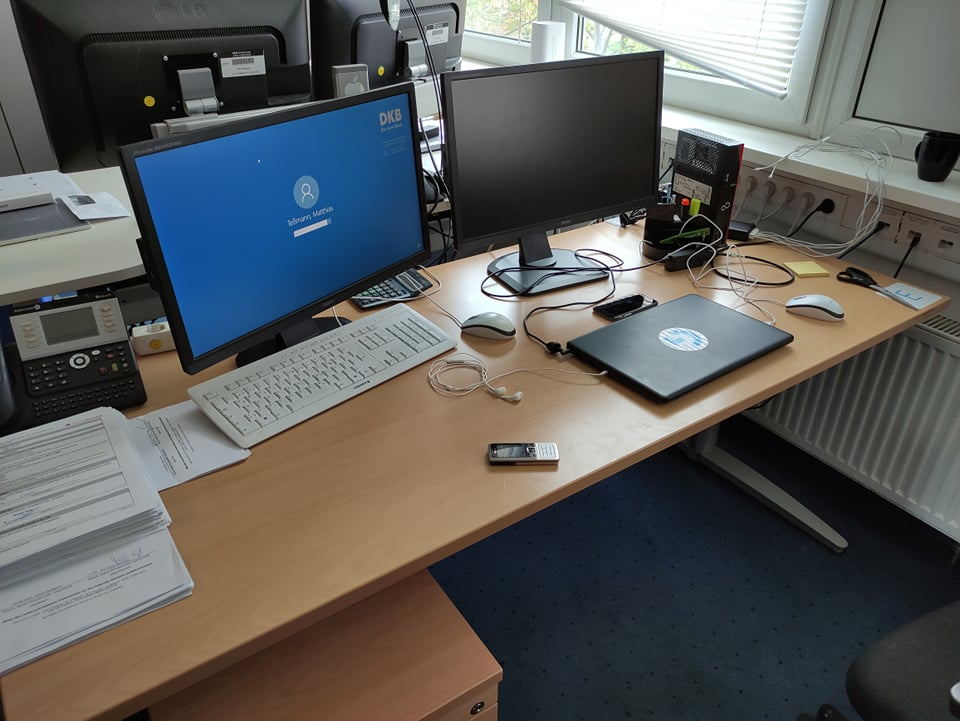
\includegraphics[width=1\textwidth]{arbeitsplatz.jpg}
  \caption{Arbeitsplatz}
  \label{fig:Bild1}
\end{figure}
\noindent
 Der Arbeitsplatz umfasste einen höhenverstellbaren Tisch, zwei Monitore und einen kleinen Stand-Pc (Thin-Client), welcher nur wenig Leistung benötigte, da sich in der DKB-Service über diese Rechner auf einer Citrix-Session eingeloggt und damit komplett arbeitsplatz-unabhängig gearbeitet werden kann. Ich bekam eine Einführung in die Hardware und den Anmeldeprozess. Danach wurden mir per E-Mail die Passwörter zu verschiedenen Programmen und Plattformen mitgeteilt. Zum Abschluss des ersten Tages bekam ich meinen Transponder, welcher sowohl als Zutrittskarte für die mechanisch gesicherten Türen im Gebäude, als auch zum Festhalten der Arbeitszeiten am Check-In dient. Die DKB-Service ermöglicht ihren Mitarbeitern übergreifend Gleitzeit als Stunden-Modell. In den darauffolgenden Arbeitstagen beschäftigte ich mich hauptsächlich mit Schulungen im Bereich IT-Sicherheit, Datensicherheit, \textit{Fraud Prevention and Detection} und Umgang mit dem Kunden. Diese Schulungen sind für jeden Mitarbeiter Pflicht und müssen alle zwei Jahre wiederholt werden. Zum Abschluss der ersten Woche bekam ich meine Hardware, welche aus einem Laptop, einem iPad 10 pro und einem iPhone 8 bestand, um auch von Zuhause arbeiten zu können. Zwischendurch bekam ich meine ersten einfachen Augaben, wobei ich besonders mit dem Updaten der iPads vertraut gemacht wurde. Diese mussten vor dem Ausliefern an die Mitarbeiter immer aktuell sein. Da die Mitarbeiter der DKB hauptsächlich mit Apple-Produkten versorgt wurden und ich bis dato kein iPhone oder Ähnliches besaß, machte ich mich ausführlich mit dem Aufbau von iOS vertraut. Die Woche verging schnell und es gelang mirl einen guten Draht zu den Kollegen aufzubauen, sodass ich mich schon auf die zweite Arbeitswoche freute.

\subsection{IT-Lager}
\label{sec:IT-Lager}

Die zweite Woche begann mit der Einführung in meinen Abreitsbereich für die ersten Wochen. Ich wurde im so genannten IT-Lager eingesetzt, wo die Laptops für Mitarbeiter der Bank mit einem hauseigenen Betriebssystem bespielt wurden.
\begin{figure}[H] 
  \centering
     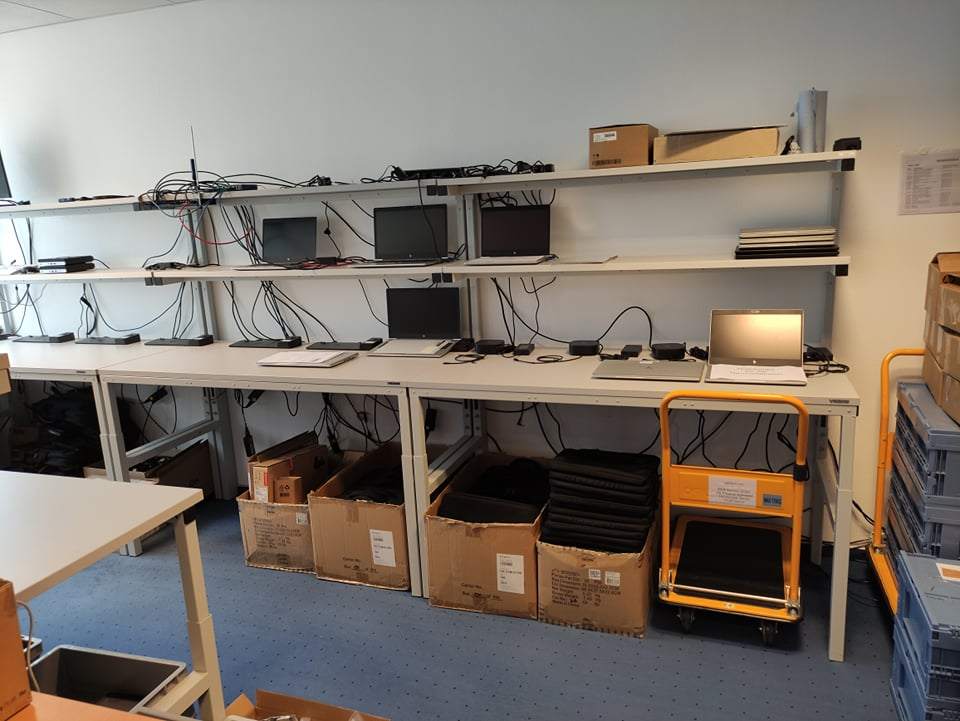
\includegraphics[width=1\textwidth]{itlager.jpg}
  \caption{IT-Lager}
  \label{fig:Bild1}
\end{figure} 
\begin{figure}[H] 
  \centering
     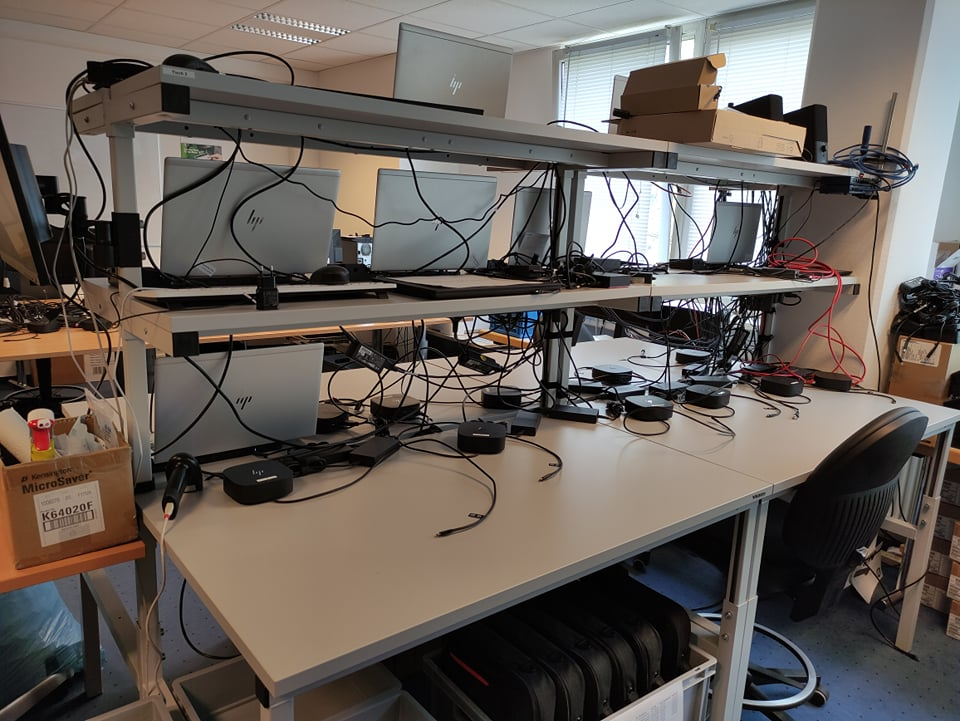
\includegraphics[width=1\textwidth]{itlager1.jpg}
  \caption{IT-Lager}
  \label{fig:Bild1}
\end{figure} 
\noindent
Des Weiteren wurden hier die Laptops gehärtet und die Festplatten verschlüsselt, sodass diese nicht missbraucht werden konnten. Ich wurde in den Ablauf des Aufsetzen eines solchen Rechners eingearbeitet, welcher im Groben daraus bestand, einen neuen Laptop an das Netzwerk anzuschließen und über einen Befehl im Bios-Terminal das Laden des Betriebssystems aus dem Netzwerk zu starten. Danach wurde auf jedem Laptop ein provisorischer Benutzer erstellt, damit die Festplatten verschlüsselt werden konnten. Es musste darauf geachtet werden, dass die Laptops keine Fehlermeldungen warfen, was durchaus vorkommen konnte. Weiterhin wurde mir beigebracht die Laptops entsprechend von Sonderanforderungen aufzurüsten, fachmännisch zu Öffnen und wieder zu Schließen. Ein solches Upgrade umfasste meist das Hinzufügen eines neuen Arbeitsspeicher-Riegels und die Erweiterung um eine neue SSD-Festplatte. Dabei war darauf zu achten sich zu erden bevor man empfindliche Hardware anfasst. Abgeschlossen wurde eine Installation des Laptops mit dem Aufspielen von Norton Security, welches den Laptop mit einem firmeneigenen Profil härtete und die Festplatten verschlüsselte. Ein weiterer Teil der Arbeit dort bestand darin die Hardware entsprechend sorgfältig zu verpacken und an die entsprechenden Mitarbeiter per Hauspost zu verschicken. Verschickt wurde die Hardware aus der Poststelle, welche gleichzeitig ein zweites kleines IT-Lager darstellte.
\begin{figure}[H] 
  \centering
     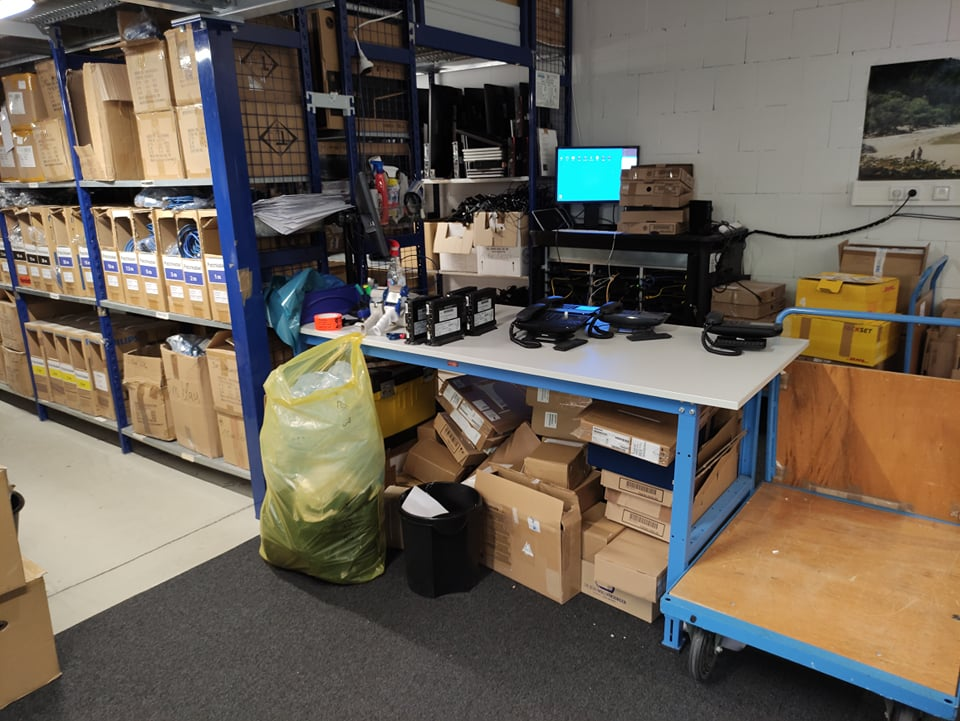
\includegraphics[width=0.9\textwidth]{poststelle.jpg}
  \caption{Poststelle}
  \label{fig:Bild1}
\end{figure} 
\begin{figure}[H] 
  \centering
     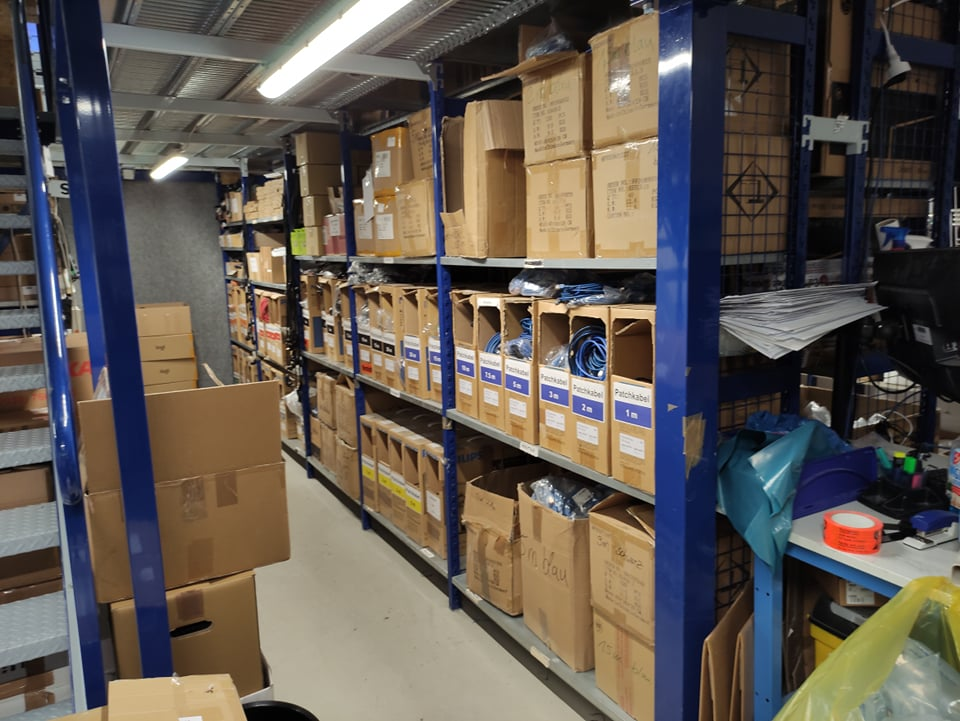
\includegraphics[width=0.9\textwidth]{poststelle1.jpg}
  \caption{Poststelle}
  \label{fig:Bild1}
\end{figure} 
\noindent

 Dort wurde kleinere zusäzliche Hardware wie LAN-Label, Router, Switches, Netzteile, Mäuse, Tastaturen und Steckdosen gelagert. In der Poststelle wurden die Etiketten zum Versand der Hardware ausgedruckt, indem im System der Mitarbeiter gesucht und dann die entsprechende Hardware verbucht wurde. Dazu wurde ein Übergabeprotokoll erstellt, welches die zu übergebenen Hardwarebestandteile auflistete. Dieses diente der Absicherung, dass auch die korrekte Hardware verschickt wurde. Der Mitarbeiter musste das Protokoll unterschreiben, einscannen und an unser Team zurückschicken. Daraufhin wurde ihm der jeweilige PIN oder Entsperrcode übermittelt, damit die Hardware verwendet werden konnte. Im spätere Verlauf versuchte ich den Prozess des Erstellens eines Übergabeprotokolls zu optimieren. Die Arbeit im IT-Lager und in der Poststelle setze das Wissen voraus welche Hardware benötigt wird und welche Ersatzteile zu den jeweiligen Geräten gehören. Dieser Teil befasste sich demnach besonders mit Hardware und den jeweiligen Komponenten. In der Poststelle gab es auch einen Bereich in dem kleinere Reperaturarbeiten an der Hardware durchgeführt werden konnten. Besonders oft benutzt ich dort den Lötkolben, mit dem ich kleinere Reperaturen an Kabeln oder gelösten Lötstellen durchführte. Dabei war besonders wichtig, dass man die richtige Spitze zu der jeweiligen Arbeit auswählte. Auch war darauf zu achten, dass das die Zusammensetzung des Lots für die entsprechende Temepratur geeignet ist und dass die Lötspitze immer sauber gehalten wird.
\\
 Ein Vorgehen beim Verlöten von Bauteilen kann folgendermaßen beschrieben werden:
\\
\begin{itemize}
	\item Die zu verbindenden Drähte verdrillen und Elektrobauelemente rutschfest auf der Platine platzieren.
	\item Ist eine solche Platzierung nicht möglich, das Bauteil mit einer Spitzzange während des Lötens fixieren.
	\item Vor dem eigentlichen Löten die Bauteile durch Berühren mit der Lötspitze auf die richtige Arbeitstemperatur bringen.
	\item Danach das Lot an die Bauteile und mit der heißen Lötspitze zum Schmelzen bringen. Das Lot sollte zwischen die Bauteile fließen, es erkaltet dann silbrig glänzend.
	\item Kommt es während des Lötens zu Erschütterungen der Lötstelle, ist die Verbindung unter Umständen nicht leitfähig. Es handelt sich um eine kalte Lötstelle, die durch Wiederholen des Lötvorgangs nachbearbeitet werden muss. Gründe für eine kalte Lötstelle können auch ein zu schwacher Lötkolben oder zu kalte Kontaktstellen der Bauteile sein. Kalte Lötstellen haben 			eine matte graue Färbung sowie eine raue Oberfläche.
	\item Reste von Lot an der Lötspitze unverzüglich entfernen.
\end{itemize}
\
\\
Zusammenfassend ist zu sagen, dass die Einarbeitungszeit besonders den hardwaretechnischen Bereich abdeckte. So lernte ich den korrekten Umgang mit sensibler Hardware, das Aufrüsten von verschiedesten Computerkomponenten, das Reparieren von einfachen Bauteilen, die Logistik hinter der Ausgabe von Hadrware und den Prozess des Aufsetzens und Härtens eines Rechners für Mitarbeiter kennen. Dieser Teil machte mir persönlich viel Spaß, da er sowohl körperliche Arbeit, als auch Präzision und Fachwissen voraussetze. Besonders die Reperaturarbeiten vermittelten mir ein solides Grundwissen, von dem ich seit dem auch privat profitieren konnte. In dieser Zeit kamen mir besonders der Einführungskurs in Computer Engineering (Löten eines USB-Sticks) und das Projekt Computer Engineering zu Gute, da dort ich dort schon einen ersten Kontakt mit Löten und den Umgang mit Bauteilen hatte. Dieses Grundwissen konnte hier erweitert und vertieft werden und es zeigt sich, dass ich mir vorstellen konnte auch beruflich in diese Richtung zu gehen, da sich diese Arbeit mehr wie ein Hobby als Arbeit anfühlte. 
\newpage

\section{Mittelfristige Projekte}
\label{sec:Mittelfristige Projekte}

Nach der Einarbeitungszeit und dem Kennenlernen der Hard- und Software wurde mir nach ca. 2 Monaten mein erstes eigenes Projekt überlassen. In diesem ging es um die ganzheitliche Planung, Organisation und Umsetzung von innerbetrieblichen Schulungen. Bei diesen Schulungen handelte es sich um SQL-, Azure-, SAP- und weitere spezielle Mitarbeiter-Schulungen. Diese Schulungen wurden regelmäßig von der DKB-Management-School geplant und finanziert. Dabei wurde in der Regel folgende Komponenten für eine Schulung benötigt:
\begin{itemize}
	\item Schulungs-Laptop
	\item Switches
	\item LAN-Kabel
	\item Netzteile
	\item Steckdosen
	\item Mäuse
\end{itemize}
\noindent
Mein Aufgabenbereich erstreckte sich von der Annahme der Tickets für Schulungen, der Beschaffung der korrekten Hardware, dem Buchen der Schulungs-Hardware, dem Verschicken der richtigen Hardware bis zur Organisation des Aufbaus beim Kunden. Im weiteren Verlauf versuchte ich den Prozess des Buchens von Hardware zu optimieren, indem ich eine eigene Buchungsseite programmierte, welche mit einer Datenbank kommunizierte die auf einem Server bei uns im Büro stand. Die Seite sollte schlicht und übersichtlich gehalten werden und wurde in Python geschrieben. Um abrufen zu können welche Laptops gebucht wurden, habe ich im weiteren Verlauf ein kleines Programm mit Benutzeroberfläche geschrieben, welches mit der Datenbank kommunizieren und die jeweiligen Einträge ausgeben und verändern konnte. So war es deutlich einfacher einen Überblick zu bekommen, welche Rechner gebucht und welche verfügbar waren. Jeder Buchung wurde das entsprechende Ticket zugeordnet und es konnte ein Blatt ausgedruckt werden, welches die genauen Hardwareanforderungen für die jeweilige Schulung enthielt. Nach einer Buchung wurde automatisch einen E-Mail mit dem Protokoll im Anhang an meine E-Mail geschickt, sodass ich sofort einen guten Überblick über die anstehende Schulung hatte. Im Prozess davor musste jeder Laptop in einer anderen Datenbank gesucht und gebucht werden. Danach musste das Übergabeprotokoll händisch ausgefüllt und ausgedruckt werden. Zudem musste irgendwo festgehalten werden, welche Laptops verschickt wurden. Der gesamte Prozess war recht unübersichtlich und beinhaltete mehrere Schritte. Durch die Ticketseite konnte der Prozess des Buchens und der Vorbereitung einer Schulung deutlich schneller durchgeführt werden. Außerdem optimierte ich die Erstellung des entsprechenden Übergabeprotokolls, welches die Korrektheit der Lieferung bestätigen sollte. Dazu implementierte ich in dem Datenbank-Programm die Funktion direkt per Knopfruck ein Übergabeprotokoll für die gebuchte Hardware zu erstellen. Während der ganzen Zeit stand mir ein Kollege zur Seite, welcher sich besonders gut mit Netzwerken und Datenbanken auskannte, sodass ich immer einen Ansprechpartner hatte. Im Bereich Datenbanken konnte ich zudem auf die Grundkenntnisse aus dem Modul Datenbanken zurückgreifen. Besonders das Wissen um die dritte Normalform und das Vermeiden von Redundanzen machte sich hier bezahlt. In Projekten in den Modulen Softwaretechnik und Datenbanken konnte ich Erfahrung in der Python-Programmierung sammeln, welche mir die Umsetzung der Projekte im Rahmen der Arbeit bei der DKB ermöglichte. Nach der erfolgreichen Buchung und Vorbereitung einer Schulung, musste ich den Aufbau organisieren. Dazu wurde eine externe Firma beauftragt, bei der es sich um die Schindler AG handelte, welche ich vor jeder Schulung mit einer Woche Vorlauf telefonisch kontaktierte und einen Aufbau koordinierte. Wenn Probleme mit den Terminen bei Schindler auftraten, dann bin ich persönlich zum jeweiligen Standort der Schulung gefahren und habe die Hardware entsprechend aufgebaut. Dabei mussten alle Laptops verkabelt, hochgefahren und betriebsbereit konfiguriert werden. Abschließend wurde ein Netzwerk aufgebaut, welches eine Kommunikation mit dem Netz der DKB gewährleistete. Dazu wurde ein oder mehrere Switches mit dem Netzwerk verbunden, indem die im Büro befindlichen Steckdosen für das Hauseigene Netzwerk verwendet wurden. Danach wurden die Laptops mit dem Switch verbunden, sodass alle auf das Netzwerk zugreifen konnten. Bei dem Netzwerk der DKB handelte es sich um zwei voneinander gekoppelte Netzwerke, welche in ein Bank- und ein Servicenetz gegliedert wurden. In einem großen Vorhaben unter dem Projektnamen Netz 4.0 sollten diese Netze miteinander fusioniert werden, was jedoch nach drei Anläufen bis heute nicht gelang. So musste meist ein Netzwerk für das Bank-Netz hergestellt werden, sodass die Schulungsmitglieder zugriff auf die SQL- oder Bank-Server hatten. Fehlerhafte Hardware musste entsprechend ausgetauscht oder repariert werden. Bei der Zusammensetzung der Hardware musste darauf geachtet werden, dass von bestimmten anfälligen Hadrwarekomponenten mehr als gefordert verschickt wurden, sodass kaputte Komponenten kompensiert werden konnten. Mit der Zeit bekam ich ein Gefühl dafür, welche Hardware oft kaputt geht. So waren es in der Regel Kabel und Netzteile, welche in der Zeit öfter kaputt gingen. Ab und zu mussten auch Switches ausgetauscht werden, was jedoch kein Problem darstellte, da ich meist zwei Switches mehr als gefordert versendete. 
\\
Es kam vor, dass Kunden besondere Anforderungen an eine Schulung hatten, welche entsprechend von mir besorgt und bereitgestellt werden mussten. Dabei ging es in der Regel mehr um Softwareanforderungen, als um Hardware. Da die Laptops entsprechend gehärtet wurden, sodass keine externen Programme einfach aufgespielt werden konnten, stellte dies oft ein Problem dar. Dieses konnte nur gelöst werden, indem ein komplett unabhängiges Betriebssystem installiert wurde, welches ein Aufspielen externer Software erlaubte. Nach Beendigung der Schulungen musste dieser Prozess wieder rückgängig gemacht werden und das alte Betriebssystem aufgespielt werden. Desweiteren musste ich entsprechende Teilnehmer-Accounts auf den Laptops einrichten, welche eine zeitliche Begrenzung hatten und jedem Mitarbeiter entsprechend zugeordnet werden konnten.
In diesem Projekt lernte ich vor allem die Kommunikation und die Zusammenarbeit mit verschiedensten Bereichen und Kollegen kennen und konnte meine Fähigkeiten im Bereich der Programmierung von Datenbanken und Web-Anwendungen verbessern und trainieren.Weiterhin wurde mein Organisationsfähigkeit und das Verständnis der Umsetzung von Hard- und Softwareanforderungen geschult. 

\subsection{Die Buchungsseite für Schulungshardware}
\label{Die Buchungsseite für Schulungshardware}

\begin{figure}[H] 
  \centering
     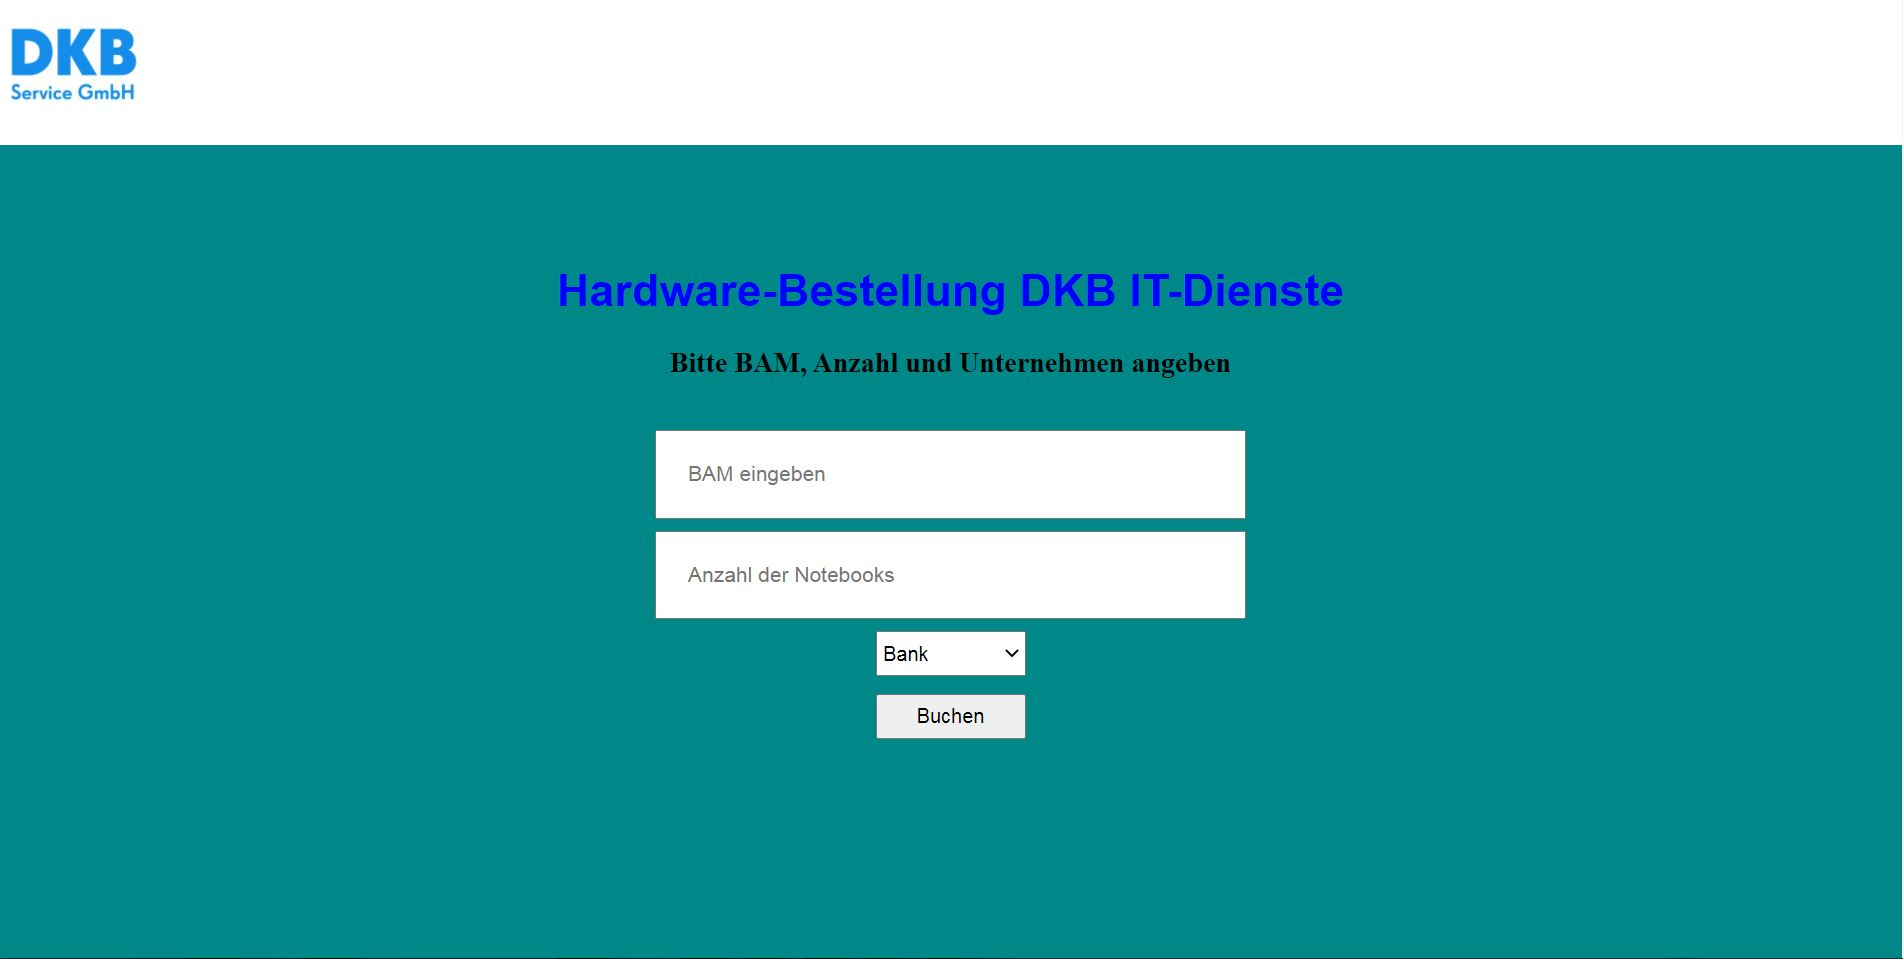
\includegraphics[width=1\textwidth]{ticketseite.jpg}
  \caption{Ticket-Seite}
  \label{fig:Bild1}
\end{figure}

\noindent
Wie auf Abbildung 1 zu erkennen ist, wurde die Seite sehr schlicht gehalten. Sie besteht aus drei HTML-Dateien, welche mit CSS \textit{gestyled} wurden. Die drei HTML-Dateien sind:

\begin{itemize}
	\item error.html
	\item index.html
	\item success.html
\end{itemize}

\noindent
Die index.html stellt die Hauptseite dar, welche beim Start angzeigt wird. Sollte einen Buchung erfolgreich sein, dann wird die nächste seite success.html und bei einem Fehler entsprechend error.html von dem Server aufgerufen. Die Datei app.py beinhaltet den Webserver und die Rendertemplate. Weiterhin wurde hier die Funktionalität des Sendens einer E-Mail bei einer Buchung aufgerufen. Es wurden folgende Bibliotheken verwendet:
\begin{itemize}
	\item flask
	\item request
	\item webbrowser
\end{itemize}

\noindent
Als Datenbank wurde eine einfache DB-Datei verwendet, welche entsprechend durch das Programm mit GUI verändert werden kann. Das Programm zum Bearbeiten der Datenbank besteht dabei aus einem Front- und einem Backend. Im Backend wurden die Funktionalitäten definiert während im Frontend die GUI gezeichnet und die Schnittstelle zwischen Backend und Datenbank geknüpft wird. In der Datenbank wurden die Latops mit Seriennummer, Name, Hersteller und Verfügbarkeit eingepflegt. Pool bedeutete dabei, dass die Laputops verfügbar waren. Über das Programm konnten der Datenbank weitere Laptops hinzugefügt oder alte bearbeitet werden.
\begin{figure}[H] 
  \centering
     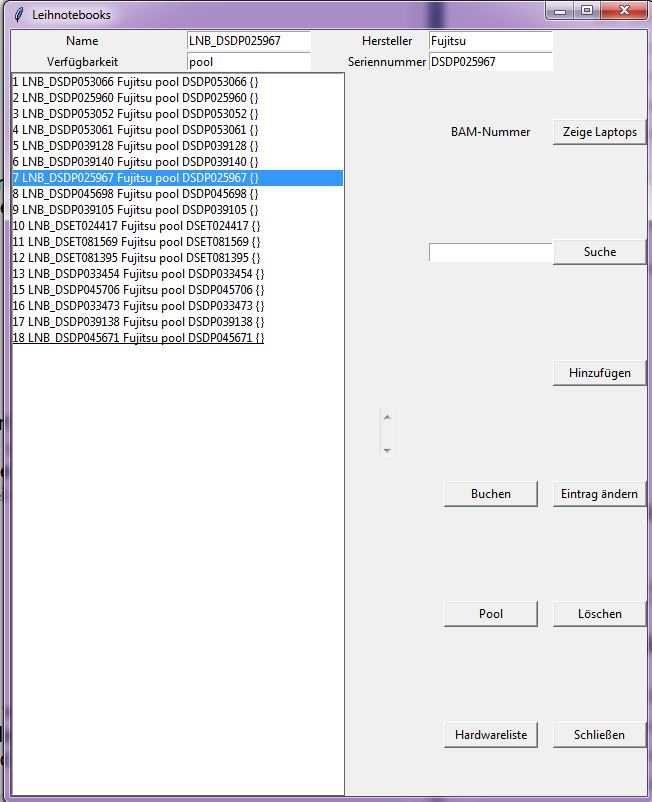
\includegraphics[width=0.7\textwidth]{frontend.jpg}
  \caption{Datenbank-Tool}
  \label{fig:Bild1}
\end{figure}

\noindent
Der Benutzer gibt auf der Ticket-Seite das BAM (Ticketnummer) zu der Bestellung im System auf der Seite an, damit diese einem Auftrag zugeordnet werden kann. Danach wird die Anzahl an benötigten Laptops eingegeben und ob es sich um das Service- oder das Banknetz handelt. Durch den Input auf dem Server werden die Funktionen des Datenbank-Tools aufgerufen und die frei verfügbaren Laptops automatisch in der Datenbank zu buchen und entsprechend auf dem Übergabeprotokoll zu vermerken. Daraufhin wird automatisch eine E-Mail mit dem entsprechenden Lieferschein, welcher die benötigte Hardware auflistet, an meine E-Mail geschickt. Die Anzahl der jeweiligen Hardwarekomponenten wird anhand von bestehenden Konventionen automatisch vom Programm erstellt und berechnet. So wurden zum Beispiel für jeweils fünf Laptops immer ein Switch verschickt. Diese Funktionalitäten wurden in attach.py implementiert, welche in die app.py importiert und von dort aufgerufen werden. 
\begin{figure}[H] 
  \centering
     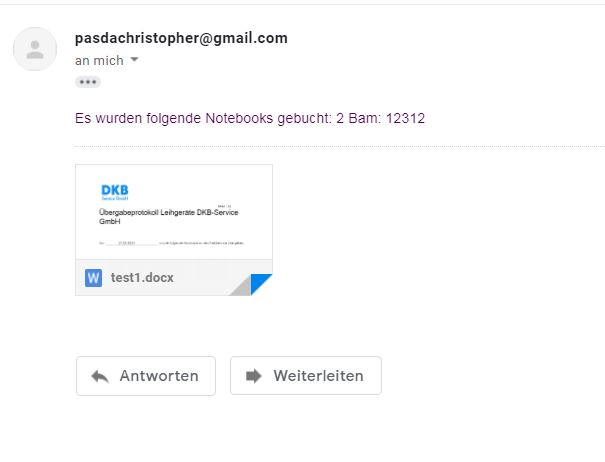
\includegraphics[width=1\textwidth]{email.jpg}
  \caption{Übergabeprotokoll}
  \label{fig:Bild1}
\end{figure}

\noindent
Um das Schicken der E-Mail und ihres Anhangs zu ermöglichen, wurde die smtplib verwendet. Bevor die E-Mail verschickt wird, wird aus der app.py über das Frontend das Übergabeprotokoll erstellt. Dazu wurden mittels der Bibliothek mailmerge Platzhalter in einem Template-Übergabeprotokoll erstellt, welche dann individuell geändert werden können. Diese werden dann mit den Daten aus der Datenbank fusioniert, umbenannt und per E-Mail verschickt.
\\

\noindent
\textbf{Fazit:}
\\ 

\noindent
In diesem Projekt konnte ich mich viel mit Python beschäftigen. Dabei wurden die Grundkenntnisse über Vektoren, For-Schleifen, Input-handling und der Umgang mit Bibliotheken vorausgesetzt. Besonders hängengeblieben sind dabei die GUI-Programmierung und der Umgang mit Datenbanken, welchen ich dank des Moduls an der HTW noch vertiefen konnte. Ich profitierte zudem von den vielen praktischen Projekten, zum Beispiel in Software Engineering, in denen ich meist Python verwendet. So konnte ich schon dort erste Erfahrungen in der Programmierung einer Benutzeroberfläche sammeln, was mir in diesem Projekt sehr zu Gute kam. Ich möchte hier erwähnen, dass sich die vielen praktischen Projekte an der HTW wirklich sehr positiv auf die Arbeit bei der DKB auswirkten und ich entsprechend froh bin, dass der Studiengang Computer Engineering so viel Praxisrelevanz zu bieten hatte. Der Code befindete sich auf dem Git-Repository.

\subsection{Projekt Serien- und Imeinummer zu Excel}
\label{Projekt Serien- und Imeinummer zu Excell}

Nach dem ersten Projekt analysierte ich Abläufe und befragte Kollegen bei welchen Prozessen ihrer Meinung nach viel Zeit verloren geht und welche deshalb optimiert werden könnten. So fand ich heraus, dass neu-gelieferte Hardware händisch eingescannt und in einer Excel-Tabelle registriert werden muss. An den Verpackungen von iPhones, iPads und Laptops befanden sich außen Barcodes (repräsentativ für die jeweilige Serial- und Imei-Nummer der Hardware), welche mittels eines Scanners eingescannt und in einer Excel-Tabelle festgehalten wurden. Diese Excel-Tabelle musste danach an Beschaffung geschickt werden, sodass diese die iPads in die Datenbank einpflegen konnten. Dieser Prozess war sehr aufwändig und zeitraubend, da die Barcodes sehr klein und schwer genau zu Treffen waren. So entschied ich mich zu versuchen mit Python und der Bibliothek Tesseract eine Bilderkennung zu programmieren, welche die Barcodes anhand eines Bildes in einer Excel-Tabelle speichern konnte, sodass lediglich ein Foto von den Barcodes eines jeden Kartons gemacht werden musste. Idealerweise sollte der erstellte Excel-Tabelle direkt an Beschaffung geschickt werden.
\begin{figure}[H] 
  \centering
     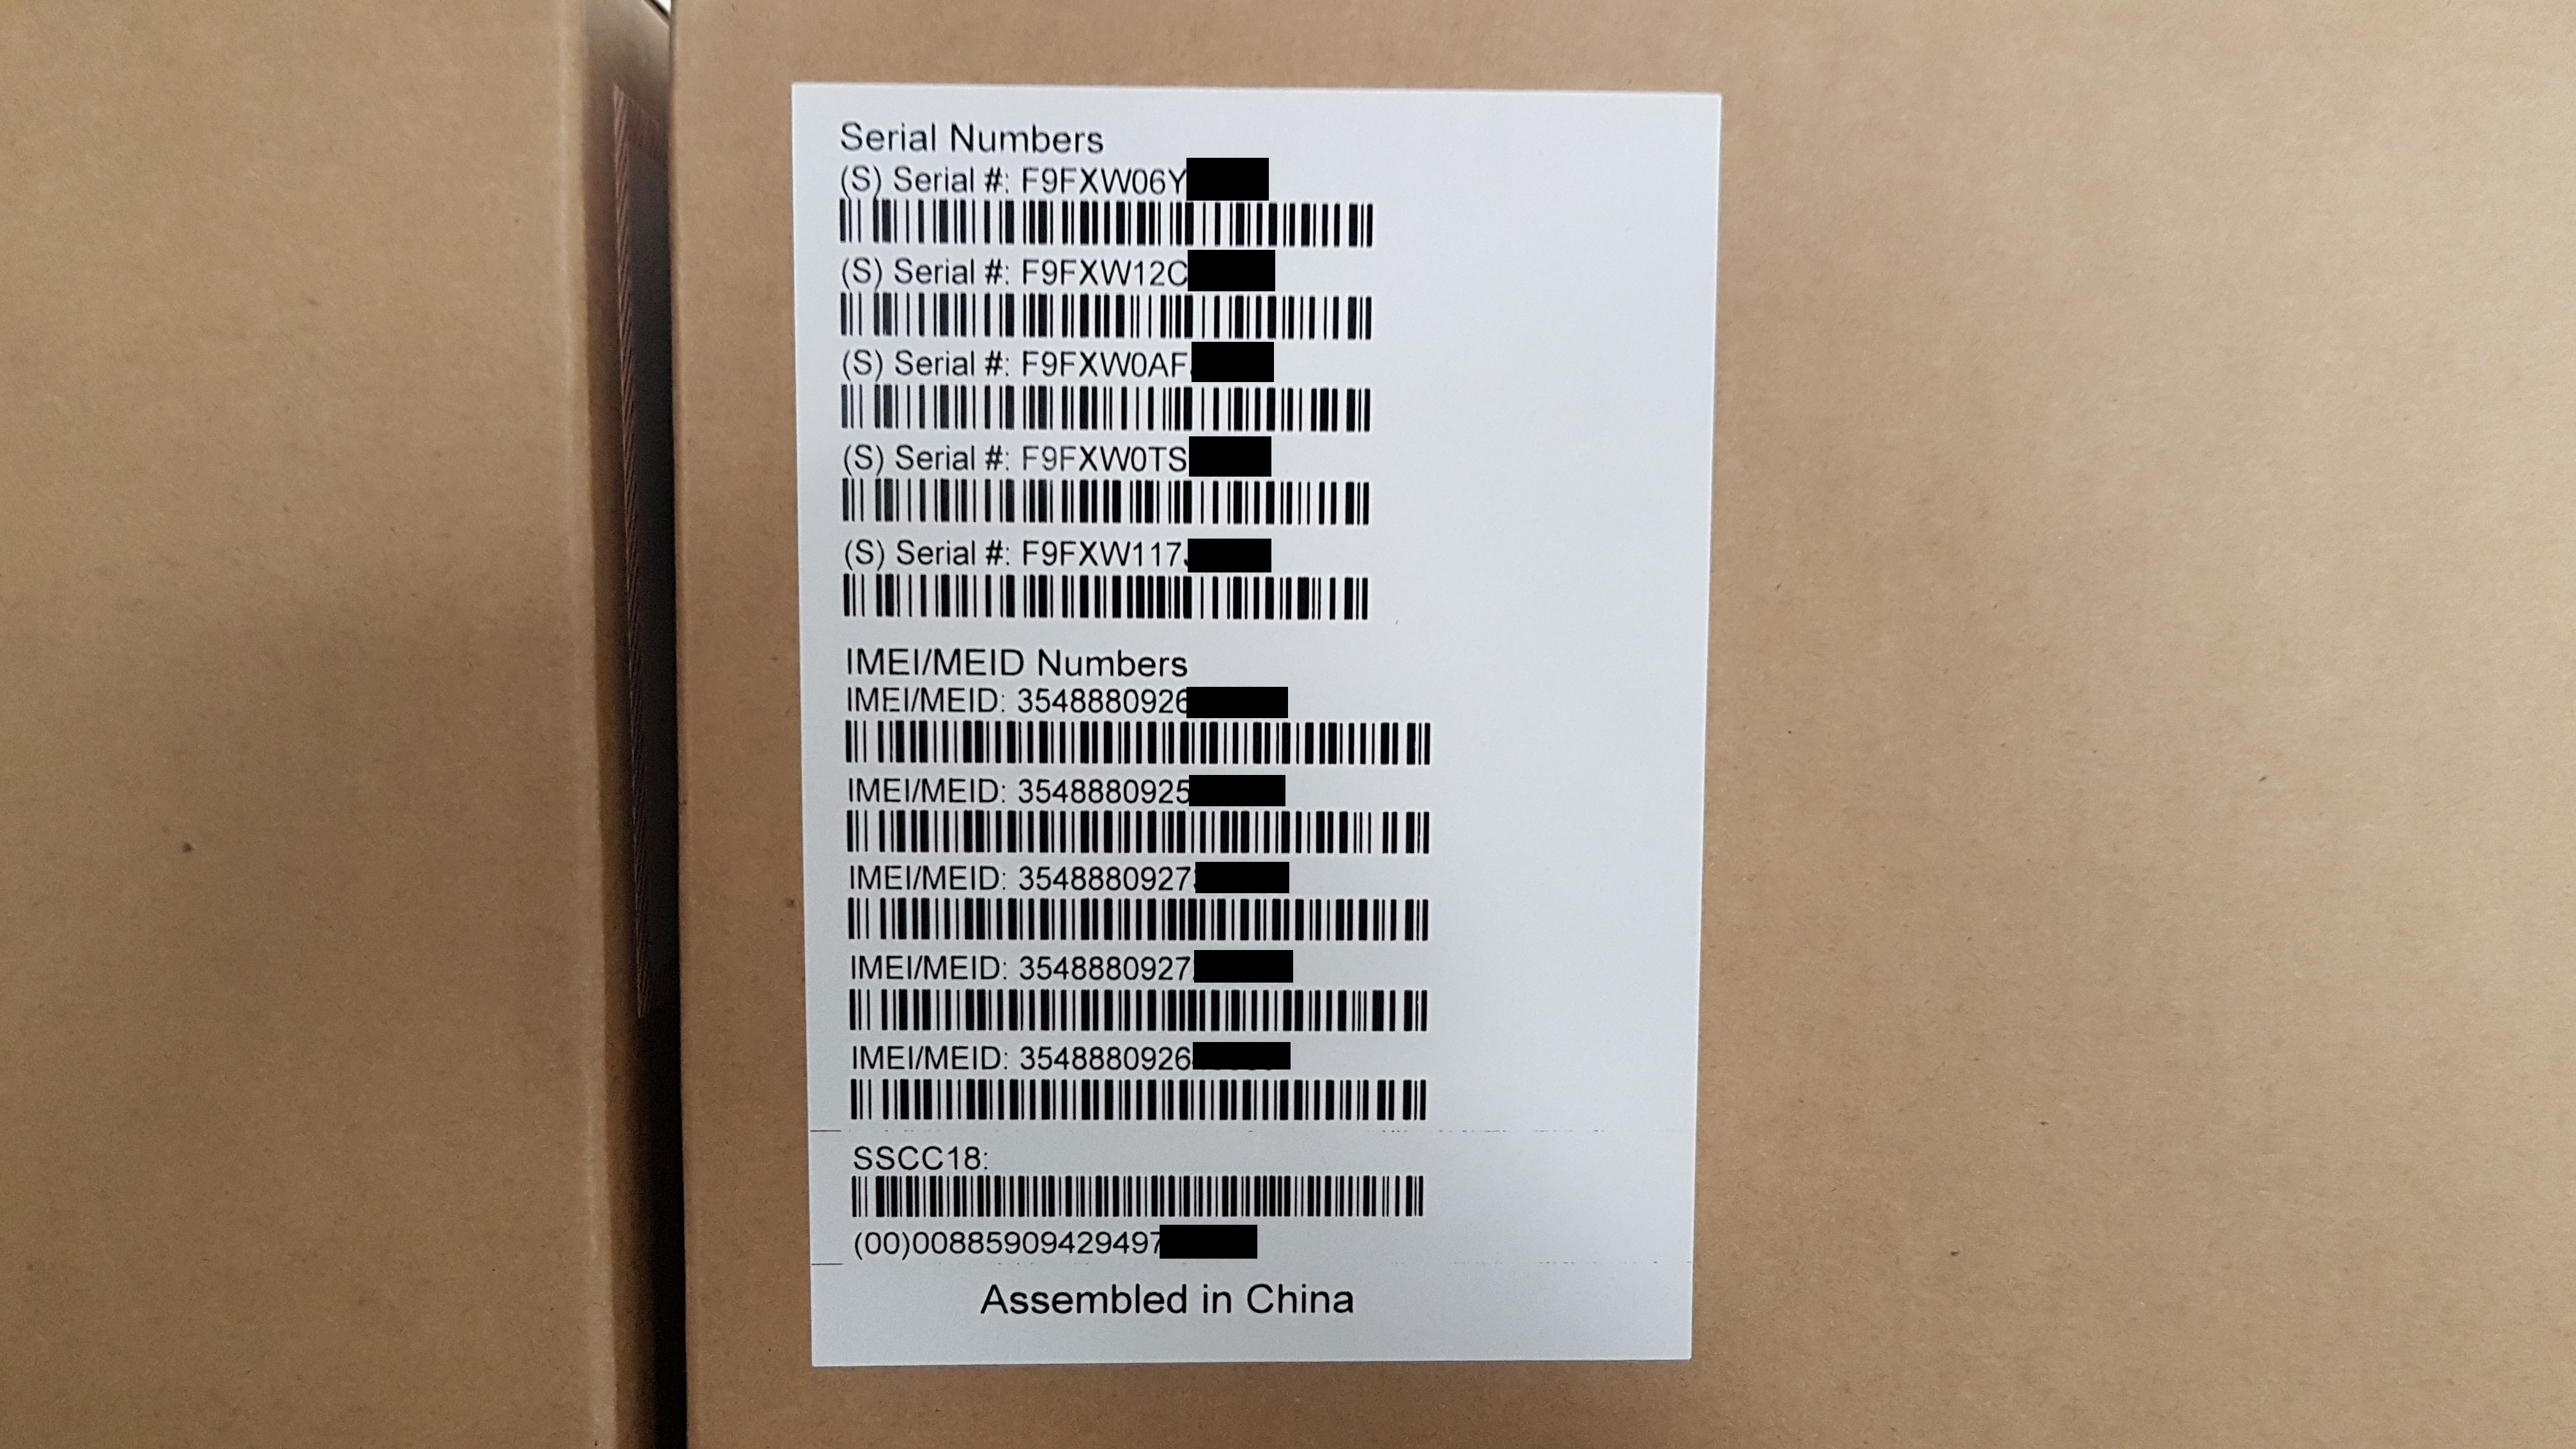
\includegraphics[width=1\textwidth]{etikett.jpg}
  \caption{Etikett iPads (zensiert aus Datenschutz)}
  \label{fig:Bild1}
\end{figure}
\noindent 
Um dies umzusetzen experimentierte ich in den ersten Wochen viel mit der Bilderkennung und der Vorverarbeitung, damit vernünftige Resultate erzielt werden konnten. Besonders wichtig bei der Texterkennung waren das Umwandeln in ein Grauwertbild, das Skallieren und Filtern des Bildes. Das Ziel dabei ist die Kanten der Ziffern zu schärfen, um so durch den Algorithmus bessere Ergebnisse zu erzielen. 
\begin{figure}[H] 
  \centering
     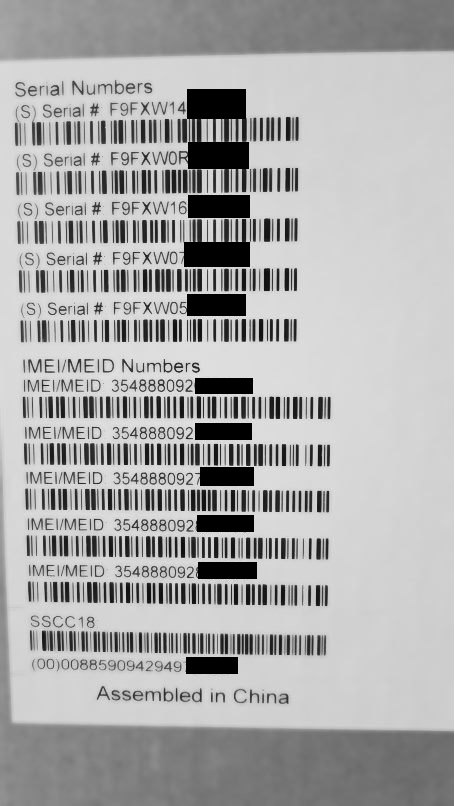
\includegraphics[width=0.4\textwidth]{serial.png}
  \caption{Vorverarbeitetes Bild}
  \label{fig:Bild1}
\end{figure}
\noindent
Dieses Bild wird der Funktion von Tesseract übergeben und daraus werden die Buchstaben mittels Algorithmus in einen String umgewandelt. Dieser String wird danach per Regex nach der Serien- und Imeinummer gefiltert und diese in einer Excel-Liste als Tupel gespeichert.
\begin{figure}[H] 
  \centering
     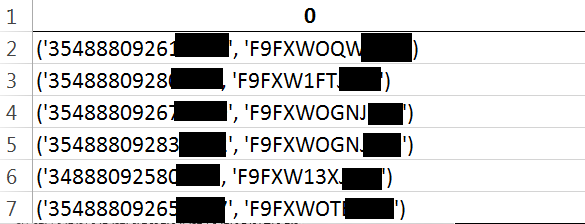
\includegraphics[width=1\textwidth]{tupel.png}
  \caption{Ergebnis als Excel-Liste}
  \label{fig:Bild1}
\end{figure}
\noindent
Aufgerufen werden die Funktion von der Hauptdatei serial.py. In diesem Script befindet sich eine While-Schleife, welche den Userinput verwaltet und die Funktionen von image.py aufruft. 
Es stellte sich heraus, dass es doch sehr schwer war ein verlässliches Ergebnis zu erzielen, bei dem wirklich jede Serien- und Imeinummer korrekt erkannt und in der Excel-Tabelle gespeichert werden konnte. Da dieser Prozess eine einhundertprozentige Zuverlässigkeit gewährleisten musste, schaffte es das Script trotz ca. 95\%iger Erkennungsrate nicht eingesetzt zu werden, da es immer wieder vorkam, dass eine Imei- oder Seriennummer nicht korrekt erkannt wurde. 
\\

\noindent
\textbf{Fazit:}
\\ 

\noindent
Während diesem Projekte lernte ich, dass es ungemein wichtig ist, dass der geschriebene Code verlässlich ist und dass man die Verantwortung trägt, wenn dabei Probleme auftreten und dass es auch sein kann, dass ein Projekt nicht im ersten Anlauf gelingt. Des weiteren verbesserte sich mein Umgang mit Python und der automatischen Bilderkennung. Der Code zu dem Script befindet sich auf dem Git. 






\newpage

\section{Weiterführende Aufgaben }
\label{sec:Weiterführende Aufgaben}

Nach der Durchführung meines ersten eigenen Projektes und der Festigung von Bindungen mit Kollegen über verschiedene Bereiche, wurde ich als vollwertiges Mitglied und Ansprechpartner in vielerlei Hinsicht angesehen. Dadurch entwickelten sich für mich eigene Aufgabengebiete, welche sich aus der Situation entwickelten, dass ich den Ruf als “Mädchen für alles” weg hatte. 

\subsection{Persönlicher Support der Führungsebene}
\label{sec:WPersönlicher Support der Führungsebene}

Bald war in der DKB bekannt, dass man bei Problemen bei mir schnell eine Lösung finden konnte, da ich neben dem Tagesgeschäft noch Kapazitäten hatte, welche dafür genutzt werden konnten. So kamen Kollegen mit einem breiten Spektrum an Problemen, welche sowohl Hardware als auch Software umfassten, zu mir und suchten Hilfe. Die häufigsten Probleme traten bei Macbooks der Grafikdesigner in der Taubenstraße auf. Dort war ich eine Zeit regelmäßig zugegen, da diese nach Updates oft Probleme bereiteten. In der Regel reichte es die Macbooks zurückzusetzen oder das Update zu deinstallieren. In dieser Zeit lernte ich besonders den Umgang mit Kollegen, Problemen und besonders die Dankbarkeit der Mitarbeiter kennen, wenn das Problem schneller behoben wurde, als gedacht. In der weiteren Zeit kamen immer wieder Kollegen mit kleineren Problemen auf mich zu, welche ich versuchte zu lösen.

\subsection{Automation von alltäglichen Aufgaben}
\label{sec:Automation von alltäglichen Aufgaben}

Besonders intensiv beschäftigte ich mich nach meinem ersten großen Projekt mit der Automation von alltäglichen Aufgaben im Büro und versucht mit Hilfe der Programmiersprache Python Abläufe zu beschleunigen und Prozesse zu vereinfachen. 
Mein erstes kleineres Projekt in diese Richtung war der Abgleich zweier Datenbanken, welche in Form von Excel-Tabellen existierten, und die Korrektur von falschen Einträgen. Diese Notwendigkeit entstand daraus, dass man die existierende Mobilfunk-Datenbank komplett erneuern wollte. In dieser Datenbank wurden die iPhones, iPads und Notebooks registriert, welche an Mitarbeiter ausgegeben wurden, sodass diese Datenbank doch sehr wichtig für das Unternehmen war. Eine Überarbeitung war notwendig, da die Datenbank über die Jahre mitgewachsen und nicht wirklich optimiert wurde, sodass die Grundlage, weaalche auf Microsoft-Access basierte, nicht mehr zeitgemäß war und es lange Ladezeiten gab. In der ersten Analyse fiel auf, dass die jeweiligen Datenbanken oft falsche Einträge aufwiesen, welche glatt gezogen werden mussten. So schrieb ich ein Programm, welches jeweils zwei Excel-Tabellen miteinander verglich und Unterschiede aufzeigte. Dies war möglich, da der Name in beiden Tabellen gleich war. Durch meine Hilfe konnten schnell Unstimmigkeiten in den jeweiligen Tabellen erkannt und behoben werden, sodass die neue Datenbank nur mit korrekten und aktuellen Einträgen gefüllt werden konnte. Danach analysierte ich Abläufe und befragte Kollegen, bei welchen Prozessen ihrer Meinung nach viel Zeit verloren ging und optimiert werden konnten. So fand ich heraus, dass neu-gelieferte Hardware händnisch eingescannt und dadurch registriert werden musste. An den Verpackungen von iPhones, iPads und Laptops befanden sich außen Barcodes(repräsentativ für die jeweilige Imei-Nummer der Hardware), welche mittels eines Scanners eingescannt und in einer Excel-Tabelle festgehalten wurden. Dieser Prozess war sehr aufwändig und zeitraubend, da die Barcodes sehr klein und schwer genau zu Treffen waren. So entschied ich mich mit Python und der Bibliothek Tesseract eine Bilderkennung zu programmieren, welche die Barcodes anhand eines Bildes in einer Excel-Tabelle speichern konnte, sodass lediglich ein Foto von den Barcodes eines jeden Kartons gemacht werden mussten. Um dies umzusetzen experimentierte ich in den ersten Wochen viel mit der Bilderkennung von der Vorverarbeitung, damit vernünftige Resultate erzielt werden konnten. Es stellte sich heraus, dass es doch sehr schwer war ein verlässliches Ergebnis zu erzielen, bei dem wirklich jede Imei korrekt erkannt und in der Excel-Tabelle gespeichert werden konnte. Da dieser Prozess eine einhundertprozentige Zuverlässigkeit gewährleisten musste, hat schaffte es das Script trotzdem 99\%iger Erkennungsrate es nicht eingesetzt zu werden, da es immer wieder vorkam, dass eine Imei nicht korrekt erkannt wurde. Während dieses kleinen Projektes lernte ich, dass es bei vielen Prozessen ungemein wichtig ist, dass der geschriebene Code verlässlich ist und dass man die Verantwortung trägt, wenn dabei Probleme auftreten. Des weiteren verbesserte sich mein Umgang mit Python und der automatischen Bilderkennung. Der Code zu dem Script befindet sich auf dem Git.

\subsection{Pflege der Datenbank}
\label{sec:Pflege der Datenbank}

Neben meinen Hauptaufgaben versuchte ich nebenbei die vorhandene Datenbank zu pflegen und eventuell falsche Einträge zu korrigieren und ein neues relationales Datenbankmodell zu entwerfen, da bei der existierenden Datenbank weder auf die dritte Normalform, noch auf andere Datenbanken-Schemata geachtet wurde, weshalb diese viele Redundanzen und Datenanomalien aufwies. Dies diente jedoch nur dem Training, da ein komplettes Team an einer komplett neuen Datenbank arbeitete. Da es sich hier um eine Nebenaufgabe handelte, welche mir eher zu Schulungszwecken diente, bekam diese Aufgabe im weiteren Verlauf immer weniger Aufmerksamkeit, sodass meine Aufmerksamkeit nach einem Monat anderen Dingen galt. Jedoch konnte ich in der Zeit mein Wissen aus dem Studien erweitern und dies auch auf eigene Datenbanken anwenden, da ich nebenbei das Modul Datenbanken belegte und ein eigenes Abschlussprojekt umgesetzt habe. 
\newpage
% einfacher Zeilenabstand



%% Index soll Stichwortverzeichnis heissen
% \newpage
% % Stichwortverzeichnis soll im Inhaltsverzeichnis auftauchen
% \addcontentsline{toc}{section}{Stichwortverzeichnis}
% \renewcommand{\indexname}{Stichwortverzeichnis}
% % Stichwortverzeichnis endgültig anzeigen
% \printindex


% evtl. Anhang


\end{document}
